\documentclass[a4paper,12pt]{article}
\usepackage{amsmath}
\usepackage{amssymb}
\usepackage[polish]{babel}
\usepackage{polski}
\usepackage[utf8]{inputenc}
\usepackage{indentfirst}
\usepackage{geometry}
\usepackage{array}
\usepackage[pdftex]{color,graphicx}
\usepackage{subfigure}
\usepackage{afterpage}
\usepackage{setspace}
\usepackage{color}
\usepackage{wrapfig}
\usepackage{listings}
\usepackage{datetime}

\renewcommand{\onehalfspacing}{\setstretch{1.6}}

\geometry{tmargin=2.5cm,bmargin=2.5cm,lmargin=2.5cm,rmargin=2.5cm}
\setlength{\parindent}{1cm}
\setlength{\parskip}{0mm}

\newenvironment{lista}{
\begin{itemize}
  \setlength{\itemsep}{1pt}
  \setlength{\parskip}{0pt}
  \setlength{\parsep}{0pt}
}{\end{itemize}}

\newcommand{\linia}{\rule{\linewidth}{0.4mm}}

\definecolor{lbcolor}{rgb}{0.95,0.95,0.95}
\lstset{
  backgroundcolor=\color{lbcolor},
  tabsize=4,
  language=C++,
  captionpos=b,
  tabsize=3,
  frame=lines,
  numbers=left,
  numberstyle=\tiny,
  numbersep=5pt,
  breaklines=true,
  showstringspaces=false,
  basicstyle=\footnotesize,
  identifierstyle=\color{magenta},
  keywordstyle=\color[rgb]{0,0,1},
  commentstyle=\color[rgb]{0,0.5,0},
  stringstyle=\color{red}
}

\begin{document}

\noindent
\begin{tabular}{|c|p{11cm}|c|} \hline
Grupa~4 & Katarzyna Kosiak i~Michał Folwarski & \ddmmyyyydate\today \tabularnewline
\hline
\end{tabular}

\section*{Zadanie~5 -- Liczby pierwsze -- MPI}
Program ma za zadanie wykonać test pierwszości (sprawdzić czy dana liczba jest liczbą pierwszą) na zestawie liczb zapisanym w~pliku.
Algorytm sprawdzania testu pierwszości został zaimplementowany na bazie metody naiwnej oraz optymalizacji~o:
\begin{lista}
 \item pominięcie liczb parzystych,
 \item pominięcie liczb podzielnych przez trzy,
 \item sprawdzenie dzielników tylko do pierwiastka kwadratowego sprawdzanej liczby.
\end{lista}

\begin{lstlisting}
if (rank == 0) { //proces glowny
    if (numberOfThreads == 1) {
        //wykonaj test pierwszosci dla wszystkich liczb
    } else {
        //rozdziel zadania
    }
} else { //pozostale procesy
    //wykonaj test pierwszosci dla otrzymanej liczby
}
\end{lstlisting}
Powyższy fragment kodu przedstawia główną ideę  w~jaki sposób zostało zorganizowane rozdzielanie zadań pomiędzy procesy w~standardzie Message Passing Interface (MPI). W~tym zadaniu równomierne rozdzielenie zadań pomiędzy dostępne procesy nie sprawdzi się, ponieważ weryfikowanie czy podana liczba jest pierwszą będzie wykonywało się w~różnym czasie. W~naszym przypadku jest to rozdzielone dynamicznie na jednoelementowe podzbiory -- każdy z~procesów (oprócz głównego) będzie otrzymywał po jednej liczbie do sprawdzenia. Dzięki takiemu podziałowi, dany proces otrzyma następne zadanie dopiero po zakończeniu poprzedniego. Zwiększanie ilości elementów w~podzbiorach powoduje, że otrzymane czasy obliczeń są nieznacznie większe lub mniejsze w~zależności od zestawu danych.

\begin{figure}[!hbp]
  \centering
    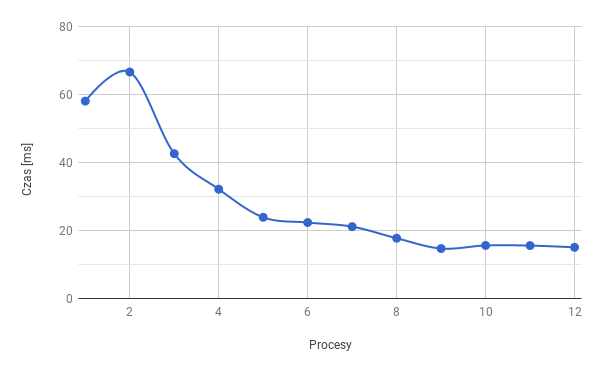
\includegraphics[width=0.7\textwidth]{chart}
  \caption{Wykres zależności czasu wykonania od ilości procesów}
  \label{chart-time-threads}
\end{figure}

Wykres na rysunku numer~1 przedstawia wyniki czasu obliczeń dla zestawu liczb znajdującym się na serwerze CUDA w~pliku \texttt{/home/shared/prir/primes/4.txt}.

Jak widać na wykresie czas wykonania dla dwóch procesów jest większy niż dla jednego, ponieważ w~naszym rozwiązaniu pierwszy proces rozdziela zadania, a~pozostałe wykonują obliczenia -- czyli dla dwóch procesów tylko jeden z~nich wykonuje właściwe obliczenia. Dodatkowy czas w~stosunku do obliczeń na jednym procesie wynika z~tego, iż do zarządzania komunikacją pomiędzy procesami oraz przydziału im zadań, potrzebna jest pewna ilości zasobów (w~tym także obliczeniowych) oraz tym, że proces który wykona sprawdzenie danej liczby pod kątem pierwszości oczekuje pewien czas otrzymanie na kolejnej liczby do sprawdzenia.

Pomimo, że na serwerze jest osiem rzeczywistych rdzeni to z~wykresu można też odczytać, że najlepszy czas obliczeń jest dla dziewięciu procesów (jeden proces rozdziela zadania, a~pozostałe osiem wykonują test pierwszości). Dzieję się to dlatego, że w~ciągu komunikacji są przerwy -- procesy obierają, przetwarzają i~wysyłają dane, a~następnie czekają na odebranie kolejnego zestawu danych. Planista systemowy zręcznie wykorzystuje to ``czekanie'' poprzez wykonanie tych zadań współbieżnie w~przeplocie.

Dalsze zwiększanie liczby procesów (ponad dziewięć) nie przynosi wzrostu przyspieszenie, a~wyniki nieznacznie się różnią od tego najlepszego.

\begin{figure}[!htbp]
  \centering
    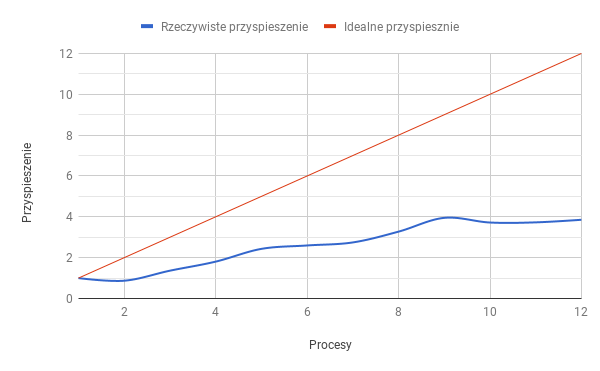
\includegraphics[width=0.7\textwidth]{chart2}
    \caption{Krzywa przyspieszenia obliczeń w~zależności od ilości procesów.}
  \label{chart-acceleration}
\end{figure}
Na rysunku numer~2 został przedstawiony wykres przyspieszenia obliczeń dla tego samego zestawu danych. Z~wykresu można odczytać, że największy przyrost szybkości obliczeń w~stosunku do obliczeń na jednym procesie jest około czterokrotny -- wyniki przyspieszenie w~dużej mierze zależą od zestawu danych i~od zaproponowanego sposobu podziału zadań pomiędzy procesami zaimplementowanego przez programistę.

\subsubsection*{Wnioski}
\noindent Dzięki zastosowaniu MPI, możliwe jest budowanie aplikacji do obliczeń równoległych za pomocą przesyłania komunikatów pomiędzy procesami. Sposób podziału zadań, wysyłania i~odbierania komunikatów należy wyłącznie do programisty -- niewątpliwie jest to trudniejsze niż w~przypadku korzystania z~OpenMP. W~tym zadaniu przetestowaliśmy możliwość dynamicznego rozdzielenia zadań pomiędzy wątki, a~co w~naszym przypadku przyniosło oczekiwane rezultaty -- obliczenia zostały zrównoleglone pomiędzy wątki i~dzięki temu zwiększyła się szybkość obliczeń.

\end{document}
